\subsection{Sekvensdiagram}
Sekvensdiagrammet viser hvordan hele programmet hænger sammen, med metodekald på tværs af klasser. 

Sekvensdigrammmet (figur \ref{fig:Sekvensdiagram}) Repræsentere en del af spillet. Dvs at ikke alle kald til alle metoder er repræsenteret.

\begin{figure}[h]
    \centering
    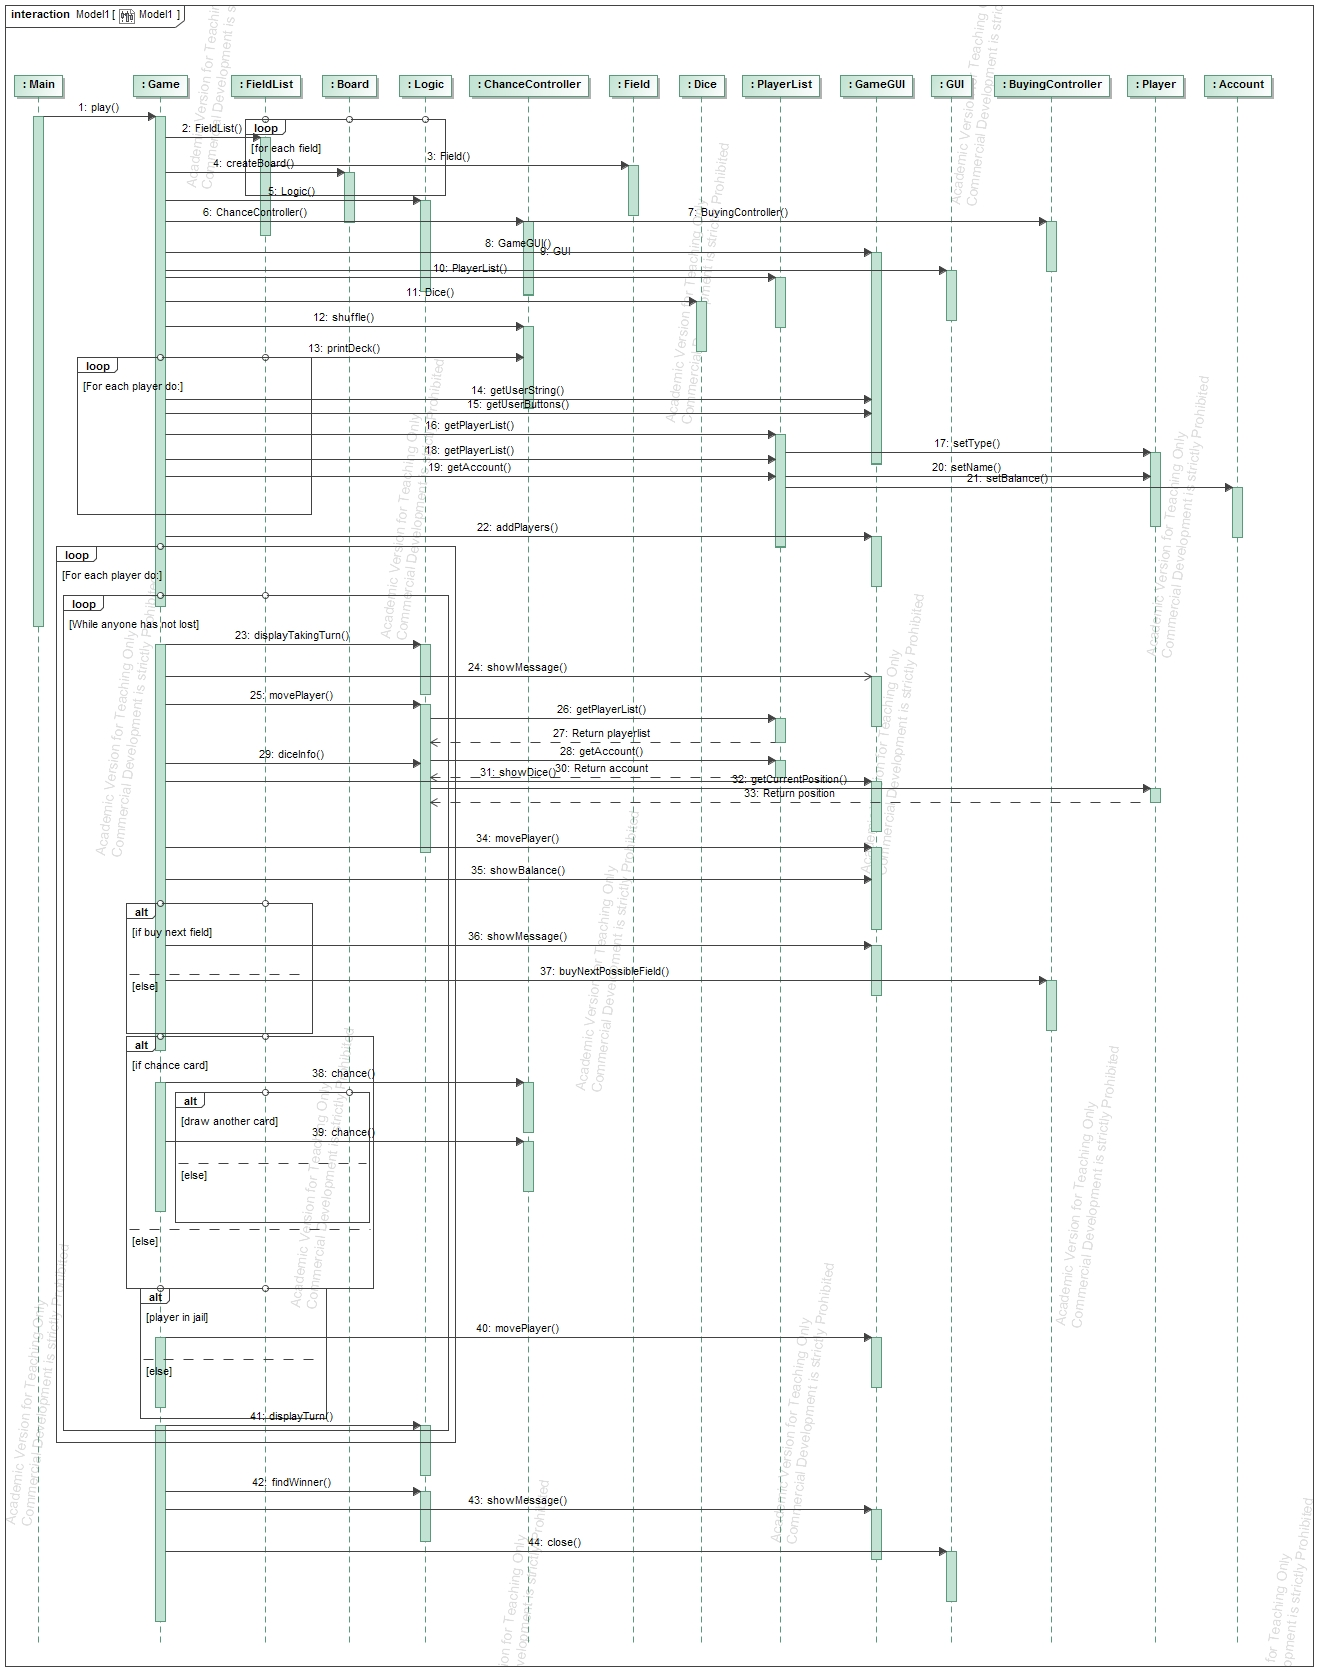
\includegraphics[width=0.7\textwidth]{sources/6_design/sekvens.jpg}
    \caption{Sekvensdiagram}
    \label{fig:Sekvensdiagram}
\end{figure}
